\chapter{Methods}
\label{mathchapter}

This part will be an overview of the overall framework of the algorithm. It
will first discuss preprocessing methods. These methods involve NMNI, NDZTA,
and error compensation in the gyroscope and accelerometer. Afterwards it will 
discuss the first and second kalman filter models, then the optional block
containing the additional sensor to improve the performance of the filter.

%%% IMU Section

\section{IMU Preprocessing}

Here I will first talk about what an IMU is, 6DOF vs. 9DOF, how each sensor
works, and the inherent errors in each sensor. 

It will then cover the planned signal processing methods for each sensor on the 
IMU and go in depth about each algorithms implementation.

\subsection{Accelerometer Signal Processing}

This subsection talks about the preprocessing methods that will take place on
the accelerometer data coming from the IMU as well as the numerical integration 
methods used for displacement calculation.

\subsubsection{Displacement Measurement from Acceleration Data}

Euler integration, trapezoidal, RK4. (Better integration = better data) 
Don't think I really need to explain this right now.

\subsubsection{No Displacement Zero Translational Accumulation (NDZTA)}

\emph{Sci-hub Link: https://sci-hub.live/https://ieeexplore.ieee.org/
document/9268038 \\ }

Removing the noise in accelerometer data during stationary points in time is 
done by finding a way to have the system understand when it is stationary. The 
No Displacement Zero Translation Accumulation (NDZTA) algorithm accounts for 
this by calculating a threshold value that indicates whether the system is in 
motion or not. Figure 2.1 illustrates the logic of the algorithm.

\begin{figure}[h]
  \centerline{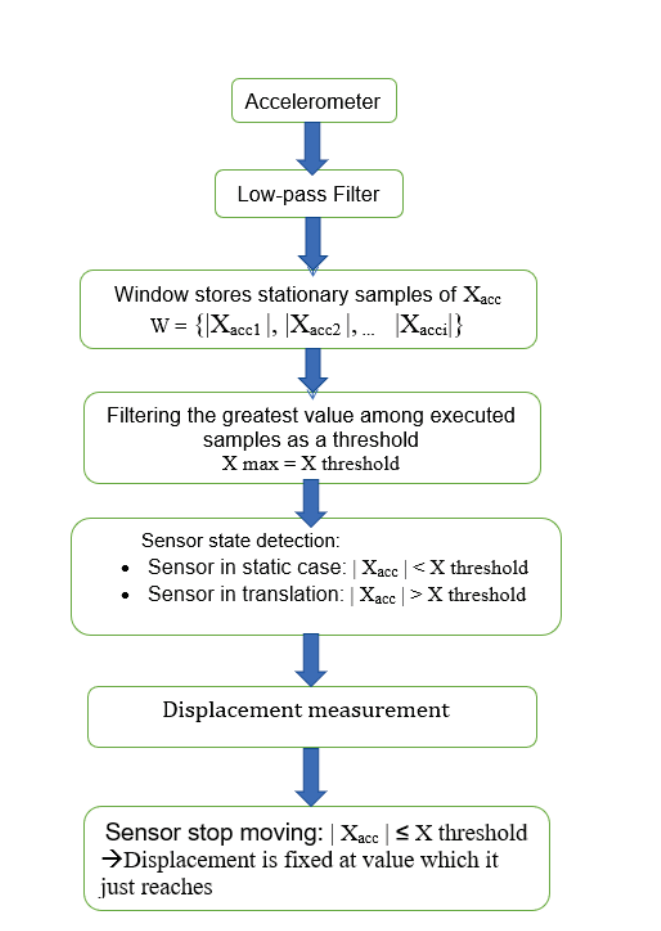
\includegraphics[height=95mm]{temp_NDZTA.PNG}}
  \caption[NDZTA Flow]{
    NDZTA flow
    }
  \label{fig:NDZTA}
\end{figure}

First a low pass filter is applied to the accelerometer data to eliminate
the inherent high frequency noise. After the filter is applied, a maximum
value is collected from a sampling window during an initial static position. 
This maximum value becomes the threshold that helps the system realize it 
is not in motion. Now the displacement is calculated based on this found 
threshold which signifies the boundary between static and dynamic motions. 
The algorithm works by comparing the real-time acceleration data $a$ with 
the threshold $a_{th}$ to decide if displacement calculation is needed. This 
comparison is demonstrated in equations 2.1 and 2.2.

\begin{equation}
	a > a_{th}, \textnormal{ Sensor is in motion. Carryout displacement calculation \\}
\end{equation}

\begin{equation}
  a \le a_{th}, \textnormal{ Sensor is static. Set acc = vel = pos = 0 \\}
\end{equation}


Note that the displacement calculation has many errors due to noise in 
the sensor signals and numerical integration causing the error to grow. In 
order to eliminate the error, the NDZTA algorithm proposes a method composed
of these 3 main steps.

\emph{ \\ Step 1: Threshold Calculation \\
 Step 2: Motion Detection \\ 
 Step 3: Displacement Measurement \\ }

During each detection of the static case, the threshold value is updated 
depending on equation 2.3.

\emph{\\ Equation 2.3 here! \\}
some conditional statement that I cannot remember.

\subsection{Gyroscope Signal Processing}

This subsection talks about the preprocessing methods that will take place on
the gyroscope data coming from the IMU.

\subsubsection{Bias Compensation}

Don't think I need to really explain this right now.

\subsubsection{No Motion No Integration (NMNI)}

\emph{Sci-hub link: https://sci-hub.live/https://ieeexplore.
ieee.org/document/9247295 \\https://sci-hub.live/https://www.sciencedirect.
com/science/article/abs/pii/S0924424721001540 \\ }

To find roll, pitch, and yaw angles, the angular rate data from the gyroscope
is numerically integrated. Due to multiple different error sources, noise 
and drift problems will cause the gyroscope data to vary. 

To compensate for these errors, the No Motion No Integration (NMNI) algorithm 
is used. This algorithm only allows numerical integration when dynamic motion
is detected. Similar to the NDZTA algorithm discussed in previous sections, 
this algorithm finds the maximum value within sampled data during an initial 
window of static motion. This max value is set as a threshold value, and 
the real-time data collected by the gyroscope is compared with the threshold 
value to determine if the system is in static or dynamic motion. The overall 
logic of the algorithm can be seen in figure 2.2 below.

\begin{figure}
  \centerline{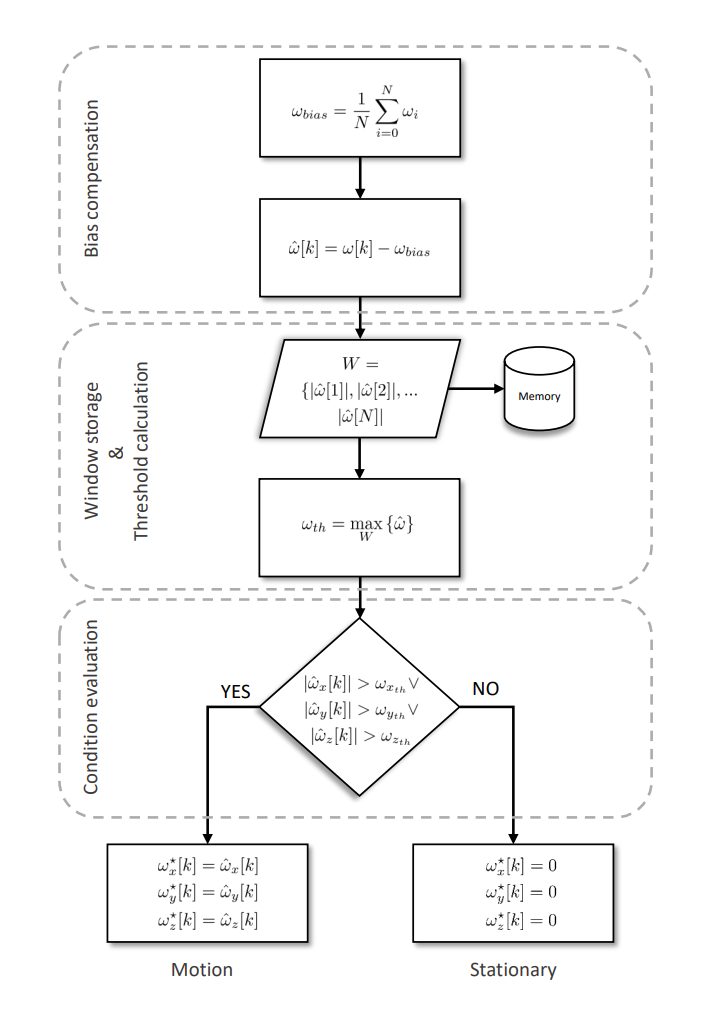
\includegraphics[height=95mm]{temp_NMNI.PNG}}
  \caption[NMNI Flow]{
    NMNI flow
    }
  \label{fig:NMNI}
\end{figure}

Maybe enter equations here too. But seems redundant.

%%%
%%% First KF block
%%%

\section{First KF: Course Correction Extended Kalman Filter}

This section covers the first Kalman Filter in the cascaded Kalman Filter framework.
This Kalman Filter uses the unicycle kinematic model as the process model, and gets
bias compensated feedback position data from the accelerometer as the measurement 
model. 

\subsection{Process Model}

The kinematic model for the robot follows the common unicycle model for a 
differentially driven wheeled-mobile robots (WMRs). This thesis is assuming 2D planar 
motion so the states are x, y, and theta. Equation 2.4 below describes the state 
transition matrix for this system. 
\\
\begin{equation}
  x = z = [x, y, \theta]^T
\end{equation}

\begin{equation}
  \dot{x} = f(x)u = 
  \begin{bmatrix}
      \cos(\theta) & 0 \\
      \sin(\theta) & 0 \\
      0 & 1
  \end{bmatrix}
  \begin{bmatrix}
      v \\
      w
  \end{bmatrix}
\end{equation}

where $v$ and $w$ are the linear and angular velocity of the mobile robot. Since we 
are working with a differential drive robot, the linear and angular velocities need 
to be related to the individual wheel speeds of the robot. The relationship 
between $v$ and $w$ and $v_L$ and $v_R$, the left and right wheel speeds of the robot 
can be seen in equations 2.5 and 2.6, where $r$ is the radius of the robot's wheel and 
$l$ is the distance between the wheels. 

\begin{equation}
  v = \frac{r}{2} (v_R + v_L)
\end{equation}

\begin{equation}
  w = \frac{r}{l} (v_R - v_L)
\end{equation}

Since this model is non-linear, the Extended Kalman Filter (EKF) is used to estimate 
the states. To implement the EKF, the Jacobian of the state transition matrix must be 
found to create a linear approximation of our non-linear equations. The EKF works by 
using a first order taylor approximation to linearize the model around the current 
state and uses the Jacobian of the model equations to calculate the covariance. To 
find the covariance, equation 2.7 is used where F is the Jacobian of the unicycle 
robot model, P is the current covariance, and Q is the process noise. 

\begin{equation}
  P^- = FPF^T + Q
\end{equation}

\begin{equation}
  F = \begin{bmatrix}
    1 & 0 & -vsin(\theta) \\
    0 & 1 &  vcos(\theta) \\
    0 & 0 &       1
  \end{bmatrix}
\end{equation}

\subsection{Measurement Model}

\begin{equation}
  z = h(x)x =  
  \begin{bmatrix}
    1 & 0 &  0 \\
    0 & 1 &  0 \\
    0 & 0 &  1
  \end{bmatrix}
  \begin{bmatrix}
    x \\
    y \\
    \theta
\end{bmatrix}
\end{equation}

The measurement model as well as its Jacobian are identity because the states can 
be directly accessed with intermediate calculations. Here the Jacobian is used to 
find the innovation covariance and can be found through equation 2.11, where $P$ is 
the covariance found from the prediction state of the Kalman filter and $R$ is the 
measurement noise.

\begin{equation}
  H = \begin{bmatrix}
    1 & 0 & 0 \\
    0 & 1 & 0 \\
    0 & 0 & 1
  \end{bmatrix}
\end{equation}

\begin{equation}
  S = HPH^T + R
\end{equation}

Going into this system will be the corrected and compensated position and 
orientation data that is found from our second Kalman Filter. In other words, the 
measurement for the first Kalman Filter is the estimation from the second Kalman 
Filter. These are then used to estimate the states taking into account the robots 
kinematic constraints along with the sensor measurements.  

To solve for heading given the gyroscope data, $w_g$ a simple Euler integration is carried 
out and can be seen in equation 2.11. 

\begin{equation}
  \theta = \theta_0 + w_g \Delta t
\end{equation}

To get global $x$ and $y$ position data from 
accelerometer readings, the local acceleration readings, $a^b$, are transformed using 
$C^g_b$ which is a rotation matrix about the z-axis, and become $a^g$, then double 
integration is carried out to arrive at global position. These conversions can be 
seen from equations 2.12-2.14. The overall conversion from the 
compensated sensor readings to the appropriate states are handled externally from 
the Kalman Filters and can be described through equations 2.11--2.14.

\begin{equation}
  a^g = C^g_b a^b
\end{equation}

\begin{equation}
  v = v_0 + a^g \Delta t
\end{equation}

\begin{equation}
  p = p_0 + v \Delta t
\end{equation}

%%%
%%% Second KF block
%%%

\section{Second KF: Bias Estimation Kalman Filter}

This section covers the second Kalman Filter in the cascaded Kalman Filter 
framework. This Kalman filter uses the gyroscope model as the process model, 
and uses the accelerometer data as the measurement model to estimate our 
states as well as correction terms to compensate for sensor errors.

\subsection{Process Model}

The states are orientation error ($\delta\phi$), velocity error ($\delta v$), 
gyroscope bias ($b_g$), and accelerometer bias ($b_a$). Each state mentioned has 3 
components relating to the north-east-down (NED) coordinate frame which gives a 
total of 12 states for the second Kalman filter.

\begin{equation}
  \boldsymbol{x}_2 = [\delta\boldsymbol{\phi}^T, \delta\boldsymbol{v}^T,
       \boldsymbol{b}^T_g, \boldsymbol{b}^T_a]^T
\end{equation}

The Kalman Filter framework and state transition matrix is one adopted from the 
popular pedestrian dead reckoning algorithm (PDR) for pedestrian rather than mobile 
robot navigation. The process model can be described through equations 2.17--2.20. 

\begin{equation}
  \delta{\dot{\boldsymbol{\phi}}} = 
  - \boldsymbol{C_b^n}\boldsymbol{b}_g^T - \boldsymbol{C_b^n}\boldsymbol{n}_g^T
\end{equation}  

The derivative of the heading error can be described by the sum of the gyro bias 
and noise, transformed into the global coordinate frame, as shown in equation 2.17.

\begin{equation}
  \delta{\dot{\boldsymbol{v}}} = 
  \boldsymbol{S}\delta\boldsymbol{\phi} + \boldsymbol{C}^n_b\boldsymbol{b}_a^T + \boldsymbol{C}^n_b\boldsymbol{n}^T_a
\end{equation}  

The derivative of the velocity error, also known as the acceleration error, is 
defined in a similar manner where it is the sum of the accelerometer noise and 
bias, transformed into the global coordinate frame, with the addition of the 
acceleration readings multipled by the previously found heading error. 

\begin{equation}
  \dot{\boldsymbol{b}}_g = 
  - \beta_g\boldsymbol{I}_{3x3}\boldsymbol{b}_g^T + \boldsymbol{I}_{3x3}w_g^T
\end{equation}  

\begin{equation}
  \dot{\boldsymbol{b}}_a = 
  - \beta_a\boldsymbol{I}_{3x3}\boldsymbol{b}_a^T + \boldsymbol{I}_{3x3}w_a^T
\end{equation}  

The derivative of the accelerometer and gyroscope bias is as a first order Gauss-Markov model,

\begin{equation}
  \dot{x} = \beta x + n
\end{equation}

where the $\beta$ values are the Markov process time constants that model our
biases. Equations 2.17--2.20 can be put together to describe our overall model 
in equation 2.22. 

\begin{equation}
  \boldsymbol{\dot{x}}_2 = \boldsymbol{f}\boldsymbol{x}_2 + \boldsymbol{g}\boldsymbol{w} = \begin{bmatrix}
        \boldsymbol{0}_{3x3} & \boldsymbol{0}_{3x3} & \boldsymbol{-C}^n_b & \boldsymbol{0}_{3x3} \\
        \boldsymbol{S} & \boldsymbol{0}_{3x3} & \boldsymbol{0}_{3x3} & \boldsymbol{C}^n_b \\
        \boldsymbol{0}_{3x3} & \boldsymbol{0}_{3x3} & -\beta_g\boldsymbol{I}_{3x3} & \boldsymbol{0}_{3x3} \\
        \boldsymbol{0}_{3x3} & \boldsymbol{0}_{3x3} & \boldsymbol{0}_{3x3} & -\beta_a\boldsymbol{I}_{3x3}
      \end{bmatrix}\boldsymbol{x_2}
      +
      \begin{bmatrix}
        \boldsymbol{-C}^n_b & \boldsymbol{0}_{3x3} & \boldsymbol{0}_{3x3} & \boldsymbol{0}_{3x3} \\
        \boldsymbol{0}_{3x3} & \boldsymbol{C}^n_b & \boldsymbol{0}_{3x3} & \boldsymbol{0}_{3x3} \\
        \boldsymbol{0}_{3x3} & \boldsymbol{0}_{3x3} & \boldsymbol{I}_{3x3} & \boldsymbol{0}_{3x3} \\
        \boldsymbol{0}_{3x3} & \boldsymbol{0}_{3x3} & \boldsymbol{0}_{3x3} & \boldsymbol{I}_{3x3}
      \end{bmatrix}\boldsymbol{w}
\end{equation}

where $\boldsymbol{C}$ is a rotation matrix representing the transformation from the local coordinate 
to global coordinates, $\boldsymbol{S}$ is a skew symmetric matrix of acceleration representing
vector cross product, and $\boldsymbol{w} = 
\begin{bmatrix}
  \boldsymbol{n_g}^T & \boldsymbol{n_a}^T & w_g^T & w_a^T \\
\end{bmatrix}^T$ is the input process noise vector. 

\begin{equation}
  \boldsymbol{C}^n_b = \begin{bmatrix}
        cos(\phi_D) & -sin(\phi_D) & 0 \\
        sin(\phi_D) &  cos(\phi_D) & 0 \\
        0 & 0 & 1 \\
      \end{bmatrix}
\end{equation}

\begin{equation}
  \boldsymbol{S} = \begin{bmatrix}
        0 & -a_D & a_E \\
        a_D & 0 & -a_N \\
        -a_E & a_N & 0 \\
      \end{bmatrix}
\end{equation}

\subsection{Measurement Model}

Measurements are course angle error and velocity measurements. Course angle error
is found by taking the difference between the previously estimated heading angle from the 
gyro and unicycle model and the estimated heading found from using the previous 
and current position data that provides the heading for the robot to linearly 
move from the previous point to the current point.

\begin{equation}
  \delta\theta = \theta_{est} - \theta_{acc}
\end{equation}

where $\theta_{est}$ is the heading estimated by the kalman filter and $\theta_{acc}$ 
is the heading found from the position data. 

\begin{equation}
  \boldsymbol{z}_2 = [\delta\theta, \boldsymbol{v}]^T
\end{equation}

\begin{equation}
  \boldsymbol{h}_2 = \begin{bmatrix}
      \begin{bmatrix}tan(\phi_N)cos(\phi_D) & tan(\phi_N)sin(\phi_D) & -1\end{bmatrix} & \boldsymbol{0}_{1x3} & \boldsymbol{0}_{1x3} & \boldsymbol{0}_{1x3} \\
      \boldsymbol{0}_{3x3} & \boldsymbol{I}_{3x3} & \boldsymbol{0}_{3x3} & \boldsymbol{0}_{3x3}
      \end{bmatrix}
\end{equation}

\section{Estimation with Additional Sensor}

This sensor should be one that can give position data. GPS, camera, encoder.
From this extra sensor, you can set up a cost function that models the error 
in the measurements and minimize it using gradient descent or something to 
hopefully get the best estimate in position/heading. 

%%%%%%%%%%%%%%%%%%%%%%%%%%%%%%%%%%%%%%%%%%%%%%%%%%%%%%%%%%%%%%%%%%

%%% Local Variables: 
%%% TeX-master: "mythesis"
%%% End: 
